\documentclass{standalone}
\usepackage{tikz}
\usetikzlibrary{patterns, positioning}

\begin{document}
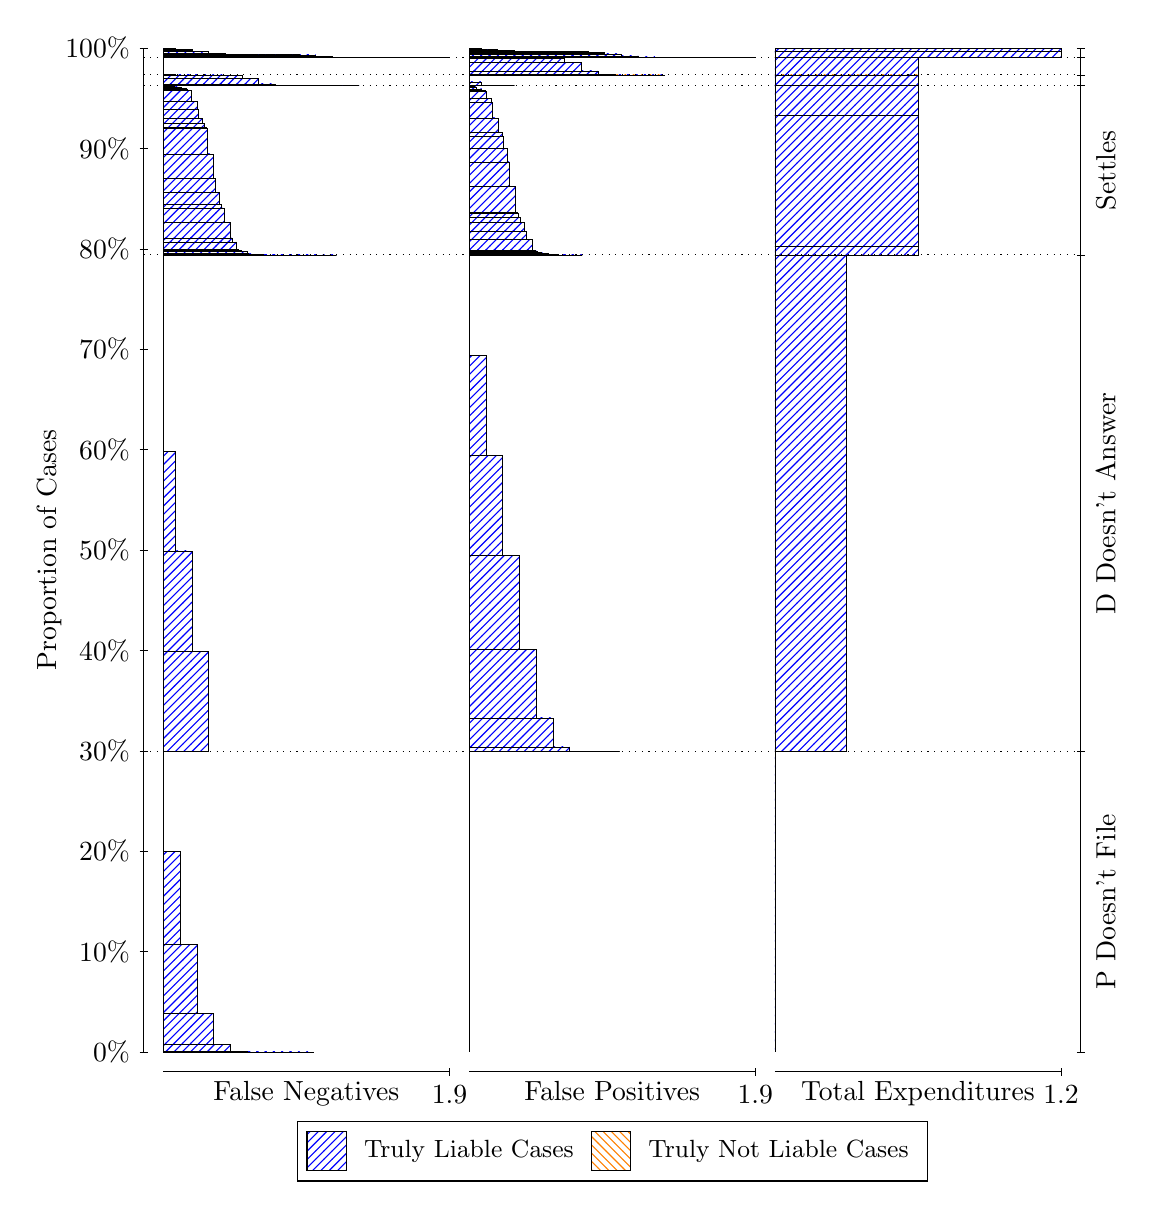
\begin{tikzpicture}
\draw[black, very thin] (1.5,1.75) -- (1.5,14.5);
\node[rotate=90, anchor=center] at (0.3, 8.125) {Proportion of Cases};
\draw[black, very thin] (1.45,1.75) -- (1.55,1.75);
\node[anchor=east] at (1.45, 1.75) {0\%};
\draw[black, very thin] (1.45,3.025) -- (1.55,3.025);
\node[anchor=east] at (1.45, 3.025) {10\%};
\draw[black, very thin] (1.45,4.3) -- (1.55,4.3);
\node[anchor=east] at (1.45, 4.3) {20\%};
\draw[black, very thin] (1.45,5.575) -- (1.55,5.575);
\node[anchor=east] at (1.45, 5.575) {30\%};
\draw[black, very thin] (1.45,6.85) -- (1.55,6.85);
\node[anchor=east] at (1.45, 6.85) {40\%};
\draw[black, very thin] (1.45,8.125) -- (1.55,8.125);
\node[anchor=east] at (1.45, 8.125) {50\%};
\draw[black, very thin] (1.45,9.4) -- (1.55,9.4);
\node[anchor=east] at (1.45, 9.4) {60\%};
\draw[black, very thin] (1.45,10.675) -- (1.55,10.675);
\node[anchor=east] at (1.45, 10.675) {70\%};
\draw[black, very thin] (1.45,11.95) -- (1.55,11.95);
\node[anchor=east] at (1.45, 11.95) {80\%};
\draw[black, very thin] (1.45,13.225) -- (1.55,13.225);
\node[anchor=east] at (1.45, 13.225) {90\%};
\draw[black, very thin] (1.45,14.5) -- (1.55,14.5);
\node[anchor=east] at (1.45, 14.5) {100\%};

\draw[black, very thin] (13.4,1.75) -- (13.4,14.5);
\draw[black, very thin] (13.35,1.75) -- (13.45,1.75);
\node[anchor=west] at (13.35, 1.75) {};
\draw[black, very thin] (13.35,5.563) -- (13.45,5.563);
\node[anchor=west] at (13.35, 5.563) {};
\draw[black, very thin] (13.35,11.874) -- (13.45,11.874);
\node[anchor=west] at (13.35, 11.874) {};
\draw[black, very thin] (13.35,14.022) -- (13.45,14.022);
\node[anchor=west] at (13.35, 14.022) {};
\draw[black, very thin] (13.35,14.159) -- (13.45,14.159);
\node[anchor=west] at (13.35, 14.159) {};
\draw[black, very thin] (13.35,14.382) -- (13.45,14.382);
\node[anchor=west] at (13.35, 14.382) {};
\draw[black, very thin] (13.35,14.5) -- (13.45,14.5);
\node[anchor=west] at (13.35, 14.5) {};

\draw[black, very thin, pattern color=blue, pattern=north east lines] (1.75,1.75) rectangle (3.6623,1.75);
\draw[black, very thin, pattern color=blue, pattern=north east lines] (1.75,1.75) rectangle (3.4498,1.75);
\draw[black, very thin, pattern color=blue, pattern=north east lines] (1.75,1.75) rectangle (3.2373,1.75);
\draw[black, very thin, pattern color=blue, pattern=north east lines] (1.75,1.75) rectangle (3.0249,1.7503);
\draw[black, very thin, pattern color=blue, pattern=north east lines] (1.75,1.7503) rectangle (2.8124,1.7582);
\draw[black, very thin, pattern color=blue, pattern=north east lines] (1.75,1.7582) rectangle (2.5999,1.8434);
\draw[black, very thin, pattern color=blue, pattern=north east lines] (1.75,1.8434) rectangle (2.3874,2.2366);
\draw[black, very thin, pattern color=blue, pattern=north east lines] (1.75,2.2366) rectangle (2.175,3.1157);
\draw[black, very thin, pattern color=blue, pattern=north east lines] (1.75,3.1157) rectangle (1.9625,4.2995);
\draw[black, very thin, pattern color=orange, pattern=north west lines] (1.75,4.2995) rectangle (1.75,4.2995);
\draw[black, very thin, pattern color=blue, pattern=north east lines] (1.75,4.2995) rectangle (1.75,5.563);
\draw[black, very thin, pattern color=blue, pattern=north east lines] (1.75,5.563) rectangle (2.3237,6.838);
\draw[black, very thin, pattern color=blue, pattern=north east lines] (1.75,6.838) rectangle (2.1112,8.1127);
\draw[black, very thin, pattern color=blue, pattern=north east lines] (1.75,8.1127) rectangle (1.8987,9.3798);
\draw[black, very thin, pattern color=orange, pattern=north west lines] (1.75,9.3798) rectangle (1.75,9.3798);
\draw[black, very thin, pattern color=blue, pattern=north east lines] (1.75,9.3798) rectangle (1.75,11.874);
\draw[black, very thin, pattern color=blue, pattern=north east lines] (1.75,11.874) rectangle (3.9491,11.874);
\draw[black, very thin, pattern color=blue, pattern=north east lines] (1.75,11.874) rectangle (3.7579,11.874);
\draw[black, very thin, pattern color=blue, pattern=north east lines] (1.75,11.874) rectangle (3.7366,11.874);
\draw[black, very thin, pattern color=blue, pattern=north east lines] (1.75,11.874) rectangle (3.6623,11.874);
\draw[black, very thin, pattern color=blue, pattern=north east lines] (1.75,11.874) rectangle (3.5667,11.874);
\draw[black, very thin, pattern color=blue, pattern=north east lines] (1.75,11.874) rectangle (3.5454,11.874);
\draw[black, very thin, pattern color=blue, pattern=north east lines] (1.75,11.874) rectangle (3.5242,11.874);
\draw[black, very thin, pattern color=blue, pattern=north east lines] (1.75,11.874) rectangle (3.4711,11.874);
\draw[black, very thin, pattern color=blue, pattern=north east lines] (1.75,11.874) rectangle (3.4498,11.874);
\draw[black, very thin, pattern color=blue, pattern=north east lines] (1.75,11.874) rectangle (3.3754,11.874);
\draw[black, very thin, pattern color=blue, pattern=north east lines] (1.75,11.874) rectangle (3.3542,11.874);
\draw[black, very thin, pattern color=blue, pattern=north east lines] (1.75,11.874) rectangle (3.3329,11.874);
\draw[black, very thin, pattern color=blue, pattern=north east lines] (1.75,11.874) rectangle (3.3117,11.874);
\draw[black, very thin, pattern color=blue, pattern=north east lines] (1.75,11.874) rectangle (3.2586,11.874);
\draw[black, very thin, pattern color=blue, pattern=north east lines] (1.75,11.874) rectangle (3.2373,11.874);
\draw[black, very thin, pattern color=blue, pattern=north east lines] (1.75,11.874) rectangle (3.163,11.874);
\draw[black, very thin, pattern color=blue, pattern=north east lines] (1.75,11.874) rectangle (3.1417,11.874);
\draw[black, very thin, pattern color=blue, pattern=north east lines] (1.75,11.874) rectangle (3.1205,11.874);
\draw[black, very thin, pattern color=blue, pattern=north east lines] (1.75,11.874) rectangle (3.0992,11.874);
\draw[black, very thin, pattern color=blue, pattern=north east lines] (1.75,11.874) rectangle (3.0461,11.874);
\draw[black, very thin, pattern color=blue, pattern=north east lines] (1.75,11.874) rectangle (3.0249,11.875);
\draw[black, very thin, pattern color=blue, pattern=north east lines] (1.75,11.875) rectangle (2.9505,11.875);
\draw[black, very thin, pattern color=blue, pattern=north east lines] (1.75,11.875) rectangle (2.9292,11.875);
\draw[black, very thin, pattern color=blue, pattern=north east lines] (1.75,11.875) rectangle (2.908,11.875);
\draw[black, very thin, pattern color=blue, pattern=north east lines] (1.75,11.875) rectangle (2.8867,11.887);
\draw[black, very thin, pattern color=blue, pattern=north east lines] (1.75,11.887) rectangle (2.8336,11.89);
\draw[black, very thin, pattern color=blue, pattern=north east lines] (1.75,11.89) rectangle (2.8124,11.913);
\draw[black, very thin, pattern color=blue, pattern=north east lines] (1.75,11.913) rectangle (2.738,11.935);
\draw[black, very thin, pattern color=blue, pattern=north east lines] (1.75,11.935) rectangle (2.7168,11.935);
\draw[black, very thin, pattern color=blue, pattern=north east lines] (1.75,11.935) rectangle (2.6955,11.943);
\draw[black, very thin, pattern color=blue, pattern=north east lines] (1.75,11.943) rectangle (2.6743,12.037);
\draw[black, very thin, pattern color=blue, pattern=north east lines] (1.75,12.037) rectangle (2.6212,12.089);
\draw[black, very thin, pattern color=blue, pattern=north east lines] (1.75,12.089) rectangle (2.5999,12.283);
\draw[black, very thin, pattern color=blue, pattern=north east lines] (1.75,12.283) rectangle (2.5255,12.464);
\draw[black, very thin, pattern color=blue, pattern=north east lines] (1.75,12.464) rectangle (2.5043,12.471);
\draw[black, very thin, pattern color=blue, pattern=north east lines] (1.75,12.471) rectangle (2.483,12.516);
\draw[black, very thin, pattern color=blue, pattern=north east lines] (1.75,12.516) rectangle (2.4618,12.674);
\draw[black, very thin, pattern color=blue, pattern=north east lines] (1.75,12.674) rectangle (2.4087,12.842);
\draw[black, very thin, pattern color=blue, pattern=north east lines] (1.75,12.842) rectangle (2.3874,13.157);
\draw[black, very thin, pattern color=blue, pattern=north east lines] (1.75,13.157) rectangle (2.3131,13.479);
\draw[black, very thin, pattern color=blue, pattern=north east lines] (1.75,13.479) rectangle (2.2918,13.495);
\draw[black, very thin, pattern color=blue, pattern=north east lines] (1.75,13.495) rectangle (2.2706,13.542);
\draw[black, very thin, pattern color=blue, pattern=north east lines] (1.75,13.542) rectangle (2.2493,13.608);
\draw[black, very thin, pattern color=blue, pattern=north east lines] (1.75,13.608) rectangle (2.1962,13.717);
\draw[black, very thin, pattern color=blue, pattern=north east lines] (1.75,13.717) rectangle (2.175,13.821);
\draw[black, very thin, pattern color=blue, pattern=north east lines] (1.75,13.821) rectangle (2.1006,13.959);
\draw[black, very thin, pattern color=blue, pattern=north east lines] (1.75,13.959) rectangle (2.0793,13.965);
\draw[black, very thin, pattern color=blue, pattern=north east lines] (1.75,13.965) rectangle (2.0581,13.973);
\draw[black, very thin, pattern color=blue, pattern=north east lines] (1.75,13.973) rectangle (2.0368,13.984);
\draw[black, very thin, pattern color=blue, pattern=north east lines] (1.75,13.984) rectangle (1.9837,13.998);
\draw[black, very thin, pattern color=blue, pattern=north east lines] (1.75,13.998) rectangle (1.9625,14.006);
\draw[black, very thin, pattern color=blue, pattern=north east lines] (1.75,14.006) rectangle (1.8881,14.02);
\draw[black, very thin, pattern color=blue, pattern=north east lines] (1.75,14.02) rectangle (1.8669,14.02);
\draw[black, very thin, pattern color=blue, pattern=north east lines] (1.75,14.02) rectangle (1.8456,14.021);
\draw[black, very thin, pattern color=blue, pattern=north east lines] (1.75,14.021) rectangle (1.7712,14.021);
\draw[black, very thin, pattern color=orange, pattern=north west lines] (1.75,14.021) rectangle (1.75,14.021);
\draw[black, very thin, pattern color=blue, pattern=north east lines] (1.75,14.021) rectangle (1.75,14.022);
\draw[black, very thin, pattern color=blue, pattern=north east lines] (1.75,14.022) rectangle (4.236,14.022);
\draw[black, very thin, pattern color=blue, pattern=north east lines] (1.75,14.022) rectangle (4.0235,14.022);
\draw[black, very thin, pattern color=blue, pattern=north east lines] (1.75,14.022) rectangle (3.811,14.022);
\draw[black, very thin, pattern color=blue, pattern=north east lines] (1.75,14.022) rectangle (3.5985,14.022);
\draw[black, very thin, pattern color=blue, pattern=north east lines] (1.75,14.022) rectangle (3.3861,14.023);
\draw[black, very thin, pattern color=blue, pattern=north east lines] (1.75,14.023) rectangle (3.1736,14.045);
\draw[black, very thin, pattern color=blue, pattern=north east lines] (1.75,14.045) rectangle (2.9611,14.112);
\draw[black, very thin, pattern color=blue, pattern=north east lines] (1.75,14.112) rectangle (2.7486,14.153);
\draw[black, very thin, pattern color=blue, pattern=north east lines] (1.75,14.153) rectangle (2.5362,14.159);
\draw[black, very thin, pattern color=blue, pattern=north east lines] (1.75,14.159) rectangle (2.3237,14.159);
\draw[black, very thin, pattern color=orange, pattern=north west lines] (1.75,14.159) rectangle (1.75,14.159);
\draw[black, very thin, pattern color=blue, pattern=north east lines] (1.75,14.159) rectangle (2.3237,14.159);
\draw[black, very thin, pattern color=blue, pattern=north east lines] (1.75,14.159) rectangle (2.1112,14.16);
\draw[black, very thin, pattern color=blue, pattern=north east lines] (1.75,14.16) rectangle (1.8987,14.167);
\draw[black, very thin, pattern color=orange, pattern=north west lines] (1.75,14.167) rectangle (1.75,14.167);
\draw[black, very thin, pattern color=blue, pattern=north east lines] (1.75,14.167) rectangle (1.75,14.382);
\draw[black, very thin, pattern color=blue, pattern=north east lines] (1.75,14.382) rectangle (5.3833,14.382);
\draw[black, very thin, pattern color=blue, pattern=north east lines] (1.75,14.382) rectangle (5.1709,14.382);
\draw[black, very thin, pattern color=blue, pattern=north east lines] (1.75,14.382) rectangle (4.9584,14.382);
\draw[black, very thin, pattern color=blue, pattern=north east lines] (1.75,14.382) rectangle (4.7459,14.382);
\draw[black, very thin, pattern color=blue, pattern=north east lines] (1.75,14.382) rectangle (4.7459,14.382);
\draw[black, very thin, pattern color=blue, pattern=north east lines] (1.75,14.382) rectangle (4.5334,14.382);
\draw[black, very thin, pattern color=blue, pattern=north east lines] (1.75,14.382) rectangle (4.5334,14.382);
\draw[black, very thin, pattern color=blue, pattern=north east lines] (1.75,14.382) rectangle (4.321,14.382);
\draw[black, very thin, pattern color=blue, pattern=north east lines] (1.75,14.382) rectangle (4.321,14.382);
\draw[black, very thin, pattern color=blue, pattern=north east lines] (1.75,14.382) rectangle (4.1085,14.383);
\draw[black, very thin, pattern color=blue, pattern=north east lines] (1.75,14.383) rectangle (4.1085,14.386);
\draw[black, very thin, pattern color=blue, pattern=north east lines] (1.75,14.386) rectangle (3.896,14.393);
\draw[black, very thin, pattern color=blue, pattern=north east lines] (1.75,14.393) rectangle (3.896,14.397);
\draw[black, very thin, pattern color=blue, pattern=north east lines] (1.75,14.397) rectangle (3.811,14.397);
\draw[black, very thin, pattern color=blue, pattern=north east lines] (1.75,14.397) rectangle (3.6835,14.412);
\draw[black, very thin, pattern color=blue, pattern=north east lines] (1.75,14.412) rectangle (3.5985,14.412);
\draw[black, very thin, pattern color=blue, pattern=north east lines] (1.75,14.412) rectangle (3.5985,14.412);
\draw[black, very thin, pattern color=blue, pattern=north east lines] (1.75,14.412) rectangle (3.4711,14.421);
\draw[black, very thin, pattern color=blue, pattern=north east lines] (1.75,14.421) rectangle (3.3861,14.421);
\draw[black, very thin, pattern color=blue, pattern=north east lines] (1.75,14.421) rectangle (3.3861,14.421);
\draw[black, very thin, pattern color=blue, pattern=north east lines] (1.75,14.421) rectangle (3.2586,14.421);
\draw[black, very thin, pattern color=blue, pattern=north east lines] (1.75,14.421) rectangle (3.2586,14.422);
\draw[black, very thin, pattern color=blue, pattern=north east lines] (1.75,14.422) rectangle (3.1736,14.422);
\draw[black, very thin, pattern color=blue, pattern=north east lines] (1.75,14.422) rectangle (3.0461,14.422);
\draw[black, very thin, pattern color=blue, pattern=north east lines] (1.75,14.422) rectangle (3.0461,14.422);
\draw[black, very thin, pattern color=blue, pattern=north east lines] (1.75,14.422) rectangle (2.9611,14.422);
\draw[black, very thin, pattern color=blue, pattern=north east lines] (1.75,14.422) rectangle (2.8336,14.422);
\draw[black, very thin, pattern color=blue, pattern=north east lines] (1.75,14.422) rectangle (2.7486,14.422);
\draw[black, very thin, pattern color=blue, pattern=north east lines] (1.75,14.422) rectangle (2.7486,14.424);
\draw[black, very thin, pattern color=blue, pattern=north east lines] (1.75,14.424) rectangle (2.6212,14.424);
\draw[black, very thin, pattern color=blue, pattern=north east lines] (1.75,14.424) rectangle (2.5362,14.424);
\draw[black, very thin, pattern color=blue, pattern=north east lines] (1.75,14.424) rectangle (2.5362,14.425);
\draw[black, very thin, pattern color=blue, pattern=north east lines] (1.75,14.425) rectangle (2.5362,14.434);
\draw[black, very thin, pattern color=blue, pattern=north east lines] (1.75,14.434) rectangle (2.5362,14.435);
\draw[black, very thin, pattern color=blue, pattern=north east lines] (1.75,14.435) rectangle (2.3237,14.435);
\draw[black, very thin, pattern color=blue, pattern=north east lines] (1.75,14.435) rectangle (2.3237,14.457);
\draw[black, very thin, pattern color=blue, pattern=north east lines] (1.75,14.457) rectangle (2.1112,14.457);
\draw[black, very thin, pattern color=blue, pattern=north east lines] (1.75,14.457) rectangle (2.1112,14.462);
\draw[black, very thin, pattern color=blue, pattern=north east lines] (1.75,14.462) rectangle (2.1112,14.471);
\draw[black, very thin, pattern color=blue, pattern=north east lines] (1.75,14.471) rectangle (2.1112,14.481);
\draw[black, very thin, pattern color=blue, pattern=north east lines] (1.75,14.481) rectangle (1.8987,14.482);
\draw[black, very thin, pattern color=blue, pattern=north east lines] (1.75,14.482) rectangle (1.8987,14.491);
\draw[black, very thin, pattern color=blue, pattern=north east lines] (1.75,14.491) rectangle (1.8987,14.494);
\draw[black, very thin, pattern color=orange, pattern=north west lines] (1.75,14.494) rectangle (1.75,14.494);
\draw[black, very thin, pattern color=blue, pattern=north east lines] (1.75,14.494) rectangle (1.75,14.5);
\draw[black, very thin, pattern color=orange, pattern=north west lines] (5.6333,1.75) rectangle (5.6333,1.75);
\draw[black, very thin, pattern color=blue, pattern=north east lines] (5.6333,1.75) rectangle (5.6333,5.563);
\draw[black, very thin, pattern color=orange, pattern=north west lines] (5.6333,5.563) rectangle (7.5456,5.563);
\draw[black, very thin, pattern color=blue, pattern=north east lines] (5.6333,5.563) rectangle (7.5456,5.563);
\draw[black, very thin, pattern color=blue, pattern=north east lines] (5.6333,5.563) rectangle (7.3331,5.563);
\draw[black, very thin, pattern color=blue, pattern=north east lines] (5.6333,5.563) rectangle (7.1207,5.5655);
\draw[black, very thin, pattern color=blue, pattern=north east lines] (5.6333,5.5655) rectangle (6.9082,5.6244);
\draw[black, very thin, pattern color=blue, pattern=north east lines] (5.6333,5.6244) rectangle (6.6957,5.9915);
\draw[black, very thin, pattern color=blue, pattern=north east lines] (5.6333,5.9915) rectangle (6.4832,6.8677);
\draw[black, very thin, pattern color=blue, pattern=north east lines] (5.6333,6.8677) rectangle (6.2708,8.0572);
\draw[black, very thin, pattern color=blue, pattern=north east lines] (5.6333,8.0572) rectangle (6.0583,9.3242);
\draw[black, very thin, pattern color=blue, pattern=north east lines] (5.6333,9.3242) rectangle (5.8458,10.599);
\draw[black, very thin, pattern color=blue, pattern=north east lines] (5.6333,10.599) rectangle (5.6333,11.874);
\draw[black, very thin, pattern color=orange, pattern=north west lines] (5.6333,11.874) rectangle (7.0675,11.874);
\draw[black, very thin, pattern color=blue, pattern=north east lines] (5.6333,11.874) rectangle (7.0675,11.874);
\draw[black, very thin, pattern color=orange, pattern=north west lines] (5.6333,11.874) rectangle (6.9719,11.874);
\draw[black, very thin, pattern color=blue, pattern=north east lines] (5.6333,11.874) rectangle (6.9719,11.874);
\draw[black, very thin, pattern color=orange, pattern=north west lines] (5.6333,11.874) rectangle (6.8763,11.874);
\draw[black, very thin, pattern color=blue, pattern=north east lines] (5.6333,11.874) rectangle (6.8763,11.874);
\draw[black, very thin, pattern color=blue, pattern=north east lines] (5.6333,11.874) rectangle (6.8551,11.874);
\draw[black, very thin, pattern color=orange, pattern=north west lines] (5.6333,11.874) rectangle (6.7807,11.874);
\draw[black, very thin, pattern color=blue, pattern=north east lines] (5.6333,11.874) rectangle (6.7807,11.874);
\draw[black, very thin, pattern color=blue, pattern=north east lines] (5.6333,11.874) rectangle (6.7595,11.875);
\draw[black, very thin, pattern color=orange, pattern=north west lines] (5.6333,11.875) rectangle (6.6851,11.875);
\draw[black, very thin, pattern color=blue, pattern=north east lines] (5.6333,11.875) rectangle (6.6851,11.875);
\draw[black, very thin, pattern color=blue, pattern=north east lines] (5.6333,11.875) rectangle (6.6638,11.876);
\draw[black, very thin, pattern color=blue, pattern=north east lines] (5.6333,11.876) rectangle (6.6426,11.89);
\draw[black, very thin, pattern color=blue, pattern=north east lines] (5.6333,11.89) rectangle (6.5682,11.898);
\draw[black, very thin, pattern color=blue, pattern=north east lines] (5.6333,11.898) rectangle (6.547,11.912);
\draw[black, very thin, pattern color=orange, pattern=north west lines] (5.6333,11.912) rectangle (6.4939,11.912);
\draw[black, very thin, pattern color=blue, pattern=north east lines] (5.6333,11.912) rectangle (6.4939,11.923);
\draw[black, very thin, pattern color=blue, pattern=north east lines] (5.6333,11.923) rectangle (6.4726,11.931);
\draw[black, very thin, pattern color=blue, pattern=north east lines] (5.6333,11.931) rectangle (6.4514,11.937);
\draw[black, very thin, pattern color=blue, pattern=north east lines] (5.6333,11.937) rectangle (6.4301,12.074);
\draw[black, very thin, pattern color=blue, pattern=north east lines] (5.6333,12.074) rectangle (6.3558,12.179);
\draw[black, very thin, pattern color=blue, pattern=north east lines] (5.6333,12.179) rectangle (6.3345,12.288);
\draw[black, very thin, pattern color=blue, pattern=north east lines] (5.6333,12.288) rectangle (6.2814,12.354);
\draw[black, very thin, pattern color=blue, pattern=north east lines] (5.6333,12.354) rectangle (6.2601,12.401);
\draw[black, very thin, pattern color=blue, pattern=north east lines] (5.6333,12.401) rectangle (6.2389,12.417);
\draw[black, very thin, pattern color=blue, pattern=north east lines] (5.6333,12.417) rectangle (6.2176,12.739);
\draw[black, very thin, pattern color=blue, pattern=north east lines] (5.6333,12.739) rectangle (6.1433,13.054);
\draw[black, very thin, pattern color=blue, pattern=north east lines] (5.6333,13.054) rectangle (6.122,13.222);
\draw[black, very thin, pattern color=blue, pattern=north east lines] (5.6333,13.222) rectangle (6.0689,13.379);
\draw[black, very thin, pattern color=blue, pattern=north east lines] (5.6333,13.379) rectangle (6.0477,13.425);
\draw[black, very thin, pattern color=blue, pattern=north east lines] (5.6333,13.425) rectangle (6.0264,13.432);
\draw[black, very thin, pattern color=blue, pattern=north east lines] (5.6333,13.432) rectangle (6.0052,13.613);
\draw[black, very thin, pattern color=blue, pattern=north east lines] (5.6333,13.613) rectangle (5.9308,13.807);
\draw[black, very thin, pattern color=blue, pattern=north east lines] (5.6333,13.807) rectangle (5.9096,13.858);
\draw[black, very thin, pattern color=blue, pattern=north east lines] (5.6333,13.858) rectangle (5.8564,13.953);
\draw[black, very thin, pattern color=blue, pattern=north east lines] (5.6333,13.953) rectangle (5.8352,13.96);
\draw[black, very thin, pattern color=blue, pattern=north east lines] (5.6333,13.96) rectangle (5.8139,13.961);
\draw[black, very thin, pattern color=blue, pattern=north east lines] (5.6333,13.961) rectangle (5.7927,13.982);
\draw[black, very thin, pattern color=blue, pattern=north east lines] (5.6333,13.982) rectangle (5.7183,14.006);
\draw[black, very thin, pattern color=blue, pattern=north east lines] (5.6333,14.006) rectangle (5.6971,14.009);
\draw[black, very thin, pattern color=blue, pattern=north east lines] (5.6333,14.009) rectangle (5.644,14.02);
\draw[black, very thin, pattern color=blue, pattern=north east lines] (5.6333,14.02) rectangle (5.6333,14.022);
\draw[black, very thin, pattern color=orange, pattern=north west lines] (5.6333,14.022) rectangle (6.207,14.022);
\draw[black, very thin, pattern color=blue, pattern=north east lines] (5.6333,14.022) rectangle (6.207,14.022);
\draw[black, very thin, pattern color=blue, pattern=north east lines] (5.6333,14.022) rectangle (5.9945,14.028);
\draw[black, very thin, pattern color=blue, pattern=north east lines] (5.6333,14.028) rectangle (5.7821,14.069);
\draw[black, very thin, pattern color=blue, pattern=north east lines] (5.6333,14.069) rectangle (5.6333,14.159);
\draw[black, very thin, pattern color=orange, pattern=north west lines] (5.6333,14.159) rectangle (8.1193,14.159);
\draw[black, very thin, pattern color=blue, pattern=north east lines] (5.6333,14.159) rectangle (8.1193,14.159);
\draw[black, very thin, pattern color=blue, pattern=north east lines] (5.6333,14.159) rectangle (7.9068,14.159);
\draw[black, very thin, pattern color=blue, pattern=north east lines] (5.6333,14.159) rectangle (7.6943,14.159);
\draw[black, very thin, pattern color=blue, pattern=north east lines] (5.6333,14.159) rectangle (7.4819,14.164);
\draw[black, very thin, pattern color=blue, pattern=north east lines] (5.6333,14.164) rectangle (7.2694,14.21);
\draw[black, very thin, pattern color=blue, pattern=north east lines] (5.6333,14.21) rectangle (7.0569,14.318);
\draw[black, very thin, pattern color=blue, pattern=north east lines] (5.6333,14.318) rectangle (6.8444,14.374);
\draw[black, very thin, pattern color=blue, pattern=north east lines] (5.6333,14.374) rectangle (6.632,14.381);
\draw[black, very thin, pattern color=blue, pattern=north east lines] (5.6333,14.381) rectangle (6.4195,14.382);
\draw[black, very thin, pattern color=blue, pattern=north east lines] (5.6333,14.382) rectangle (6.207,14.382);
\draw[black, very thin, pattern color=orange, pattern=north west lines] (5.6333,14.382) rectangle (9.2667,14.382);
\draw[black, very thin, pattern color=blue, pattern=north east lines] (5.6333,14.382) rectangle (9.2667,14.382);
\draw[black, very thin, pattern color=orange, pattern=north west lines] (5.6333,14.382) rectangle (9.0542,14.382);
\draw[black, very thin, pattern color=blue, pattern=north east lines] (5.6333,14.382) rectangle (9.0542,14.382);
\draw[black, very thin, pattern color=orange, pattern=north west lines] (5.6333,14.382) rectangle (8.8417,14.382);
\draw[black, very thin, pattern color=blue, pattern=north east lines] (5.6333,14.382) rectangle (8.8417,14.382);
\draw[black, very thin, pattern color=blue, pattern=north east lines] (5.6333,14.382) rectangle (8.6292,14.382);
\draw[black, very thin, pattern color=orange, pattern=north west lines] (5.6333,14.382) rectangle (8.6292,14.382);
\draw[black, very thin, pattern color=blue, pattern=north east lines] (5.6333,14.382) rectangle (8.6292,14.382);
\draw[black, very thin, pattern color=orange, pattern=north west lines] (5.6333,14.382) rectangle (8.4168,14.382);
\draw[black, very thin, pattern color=blue, pattern=north east lines] (5.6333,14.382) rectangle (8.4168,14.382);
\draw[black, very thin, pattern color=blue, pattern=north east lines] (5.6333,14.382) rectangle (8.4168,14.382);
\draw[black, very thin, pattern color=orange, pattern=north west lines] (5.6333,14.382) rectangle (8.2043,14.382);
\draw[black, very thin, pattern color=blue, pattern=north east lines] (5.6333,14.382) rectangle (8.2043,14.383);
\draw[black, very thin, pattern color=blue, pattern=north east lines] (5.6333,14.383) rectangle (8.2043,14.383);
\draw[black, very thin, pattern color=blue, pattern=north east lines] (5.6333,14.383) rectangle (7.9918,14.383);
\draw[black, very thin, pattern color=orange, pattern=north west lines] (5.6333,14.383) rectangle (7.9918,14.383);
\draw[black, very thin, pattern color=blue, pattern=north east lines] (5.6333,14.383) rectangle (7.9918,14.387);
\draw[black, very thin, pattern color=orange, pattern=north west lines] (5.6333,14.387) rectangle (7.7793,14.387);
\draw[black, very thin, pattern color=blue, pattern=north east lines] (5.6333,14.387) rectangle (7.7793,14.393);
\draw[black, very thin, pattern color=blue, pattern=north east lines] (5.6333,14.393) rectangle (7.7793,14.401);
\draw[black, very thin, pattern color=blue, pattern=north east lines] (5.6333,14.401) rectangle (7.5669,14.419);
\draw[black, very thin, pattern color=blue, pattern=north east lines] (5.6333,14.419) rectangle (7.5669,14.425);
\draw[black, very thin, pattern color=blue, pattern=north east lines] (5.6333,14.425) rectangle (7.3544,14.427);
\draw[black, very thin, pattern color=blue, pattern=north east lines] (5.6333,14.427) rectangle (7.3544,14.446);
\draw[black, very thin, pattern color=blue, pattern=north east lines] (5.6333,14.446) rectangle (7.3544,14.447);
\draw[black, very thin, pattern color=blue, pattern=north east lines] (5.6333,14.447) rectangle (7.1419,14.452);
\draw[black, very thin, pattern color=blue, pattern=north east lines] (5.6333,14.452) rectangle (7.1419,14.453);
\draw[black, very thin, pattern color=blue, pattern=north east lines] (5.6333,14.453) rectangle (7.1419,14.457);
\draw[black, very thin, pattern color=blue, pattern=north east lines] (5.6333,14.457) rectangle (7.1419,14.457);
\draw[black, very thin, pattern color=orange, pattern=north west lines] (5.6333,14.457) rectangle (7.0569,14.457);
\draw[black, very thin, pattern color=blue, pattern=north east lines] (5.6333,14.457) rectangle (7.0569,14.457);
\draw[black, very thin, pattern color=blue, pattern=north east lines] (5.6333,14.457) rectangle (6.9294,14.459);
\draw[black, very thin, pattern color=blue, pattern=north east lines] (5.6333,14.459) rectangle (6.9294,14.459);
\draw[black, very thin, pattern color=blue, pattern=north east lines] (5.6333,14.459) rectangle (6.9294,14.46);
\draw[black, very thin, pattern color=orange, pattern=north west lines] (5.6333,14.46) rectangle (6.8444,14.46);
\draw[black, very thin, pattern color=blue, pattern=north east lines] (5.6333,14.46) rectangle (6.8444,14.46);
\draw[black, very thin, pattern color=blue, pattern=north east lines] (5.6333,14.46) rectangle (6.717,14.46);
\draw[black, very thin, pattern color=blue, pattern=north east lines] (5.6333,14.46) rectangle (6.717,14.46);
\draw[black, very thin, pattern color=blue, pattern=north east lines] (5.6333,14.46) rectangle (6.717,14.46);
\draw[black, very thin, pattern color=blue, pattern=north east lines] (5.6333,14.46) rectangle (6.632,14.46);
\draw[black, very thin, pattern color=orange, pattern=north west lines] (5.6333,14.46) rectangle (6.632,14.46);
\draw[black, very thin, pattern color=blue, pattern=north east lines] (5.6333,14.46) rectangle (6.632,14.46);
\draw[black, very thin, pattern color=blue, pattern=north east lines] (5.6333,14.46) rectangle (6.5045,14.46);
\draw[black, very thin, pattern color=blue, pattern=north east lines] (5.6333,14.46) rectangle (6.5045,14.46);
\draw[black, very thin, pattern color=blue, pattern=north east lines] (5.6333,14.46) rectangle (6.5045,14.46);
\draw[black, very thin, pattern color=blue, pattern=north east lines] (5.6333,14.46) rectangle (6.4195,14.461);
\draw[black, very thin, pattern color=orange, pattern=north west lines] (5.6333,14.461) rectangle (6.4195,14.461);
\draw[black, very thin, pattern color=blue, pattern=north east lines] (5.6333,14.461) rectangle (6.4195,14.461);
\draw[black, very thin, pattern color=blue, pattern=north east lines] (5.6333,14.461) rectangle (6.4195,14.461);
\draw[black, very thin, pattern color=blue, pattern=north east lines] (5.6333,14.461) rectangle (6.292,14.461);
\draw[black, very thin, pattern color=blue, pattern=north east lines] (5.6333,14.461) rectangle (6.292,14.461);
\draw[black, very thin, pattern color=blue, pattern=north east lines] (5.6333,14.461) rectangle (6.207,14.466);
\draw[black, very thin, pattern color=orange, pattern=north west lines] (5.6333,14.466) rectangle (6.207,14.466);
\draw[black, very thin, pattern color=blue, pattern=north east lines] (5.6333,14.466) rectangle (6.207,14.469);
\draw[black, very thin, pattern color=blue, pattern=north east lines] (5.6333,14.469) rectangle (6.207,14.47);
\draw[black, very thin, pattern color=blue, pattern=north east lines] (5.6333,14.47) rectangle (6.0795,14.47);
\draw[black, very thin, pattern color=blue, pattern=north east lines] (5.6333,14.47) rectangle (6.0795,14.47);
\draw[black, very thin, pattern color=blue, pattern=north east lines] (5.6333,14.47) rectangle (5.9945,14.482);
\draw[black, very thin, pattern color=blue, pattern=north east lines] (5.6333,14.482) rectangle (5.9945,14.485);
\draw[black, very thin, pattern color=blue, pattern=north east lines] (5.6333,14.485) rectangle (5.8671,14.485);
\draw[black, very thin, pattern color=blue, pattern=north east lines] (5.6333,14.485) rectangle (5.7821,14.485);
\draw[black, very thin, pattern color=blue, pattern=north east lines] (5.6333,14.485) rectangle (5.7821,14.49);
\draw[black, very thin, pattern color=blue, pattern=north east lines] (5.6333,14.49) rectangle (5.7821,14.495);
\draw[black, very thin, pattern color=blue, pattern=north east lines] (5.6333,14.495) rectangle (5.6333,14.5);
\draw[black, very thin, pattern color=orange, pattern=north west lines] (9.5167,1.75) rectangle (9.5167,1.75);
\draw[black, very thin, pattern color=blue, pattern=north east lines] (9.5167,1.75) rectangle (9.5167,5.563);
\draw[black, very thin, pattern color=orange, pattern=north west lines] (9.5167,5.563) rectangle (10.425,5.563);
\draw[black, very thin, pattern color=blue, pattern=north east lines] (9.5167,5.563) rectangle (10.425,11.874);
\draw[black, very thin, pattern color=orange, pattern=north west lines] (9.5167,11.874) rectangle (11.333,11.874);
\draw[black, very thin, pattern color=blue, pattern=north east lines] (9.5167,11.874) rectangle (11.333,11.982);
\draw[black, very thin, pattern color=orange, pattern=north west lines] (9.5167,11.982) rectangle (11.333,11.982);
\draw[black, very thin, pattern color=blue, pattern=north east lines] (9.5167,11.982) rectangle (11.333,13.647);
\draw[black, very thin, pattern color=orange, pattern=north west lines] (9.5167,13.647) rectangle (11.333,13.647);
\draw[black, very thin, pattern color=blue, pattern=north east lines] (9.5167,13.647) rectangle (11.333,14.022);
\draw[black, very thin, pattern color=orange, pattern=north west lines] (9.5167,14.022) rectangle (11.333,14.022);
\draw[black, very thin, pattern color=blue, pattern=north east lines] (9.5167,14.022) rectangle (11.333,14.159);
\draw[black, very thin, pattern color=orange, pattern=north west lines] (9.5167,14.159) rectangle (11.333,14.159);
\draw[black, very thin, pattern color=blue, pattern=north east lines] (9.5167,14.159) rectangle (11.333,14.382);
\draw[black, very thin, pattern color=orange, pattern=north west lines] (9.5167,14.382) rectangle (13.15,14.382);
\draw[black, very thin, pattern color=blue, pattern=north east lines] (9.5167,14.382) rectangle (13.15,14.455);
\draw[black, very thin, pattern color=orange, pattern=north west lines] (9.5167,14.455) rectangle (13.15,14.455);
\draw[black, very thin, pattern color=blue, pattern=north east lines] (9.5167,14.455) rectangle (13.15,14.5);
\draw[black, dotted] (1.5,5.563) -- (13.4,5.563);
\draw[black, dotted] (1.5,11.874) -- (13.4,11.874);
\draw[black, dotted] (1.5,14.022) -- (13.4,14.022);
\draw[black, dotted] (1.5,14.159) -- (13.4,14.159);
\draw[black, dotted] (1.5,14.382) -- (13.4,14.382);
\draw[black, very thin] (1.75,1.5) -- (5.3833,1.5);
\node[anchor=north] at (3.5667, 1.5) {False Negatives};
\draw[black, very thin] (5.3833,1.45) -- (5.3833,1.55);
\node[anchor=north] at (5.3833, 1.45) {1.9};

\draw[black, very thin] (5.6333,1.5) -- (9.2667,1.5);
\node[anchor=north] at (7.45, 1.5) {False Positives};
\draw[black, very thin] (9.2667,1.45) -- (9.2667,1.55);
\node[anchor=north] at (9.2667, 1.45) {1.9};

\draw[black, very thin] (9.5167,1.5) -- (13.15,1.5);
\node[anchor=north] at (11.333, 1.5) {Total Expenditures};
\draw[black, very thin] (13.15,1.45) -- (13.15,1.55);
\node[anchor=north] at (13.15, 1.45) {1.2};

\node[black, centered, rotate=90] at (13.72, 3.6565) {P Doesn't File};
\node[black, centered, rotate=90] at (13.72, 8.7185) {D Doesn't Answer};
\node[black, centered, rotate=90] at (13.72, 12.948) {Settles};




\draw (7.449999999999999,1.5) node[draw=none] (baseCoordinate) {};
\begin{scope}[align=center]
        \matrix[scale=0.5, draw=black, below=0.5cm of baseCoordinate, nodes={draw}, column sep=0.1cm]{
            \node[rectangle, draw, minimum width=0.5cm, minimum height=0.5cm, pattern=north east lines, pattern color=blue] {}; &
            \node[draw=none, font=\small] (B) {Truly Liable Cases}; &
            \node[rectangle, draw, minimum width=0.5cm, minimum height=0.5cm, pattern=north west lines, pattern color=orange] {}; &
            \node[draw=none, font=\small] (B) {Truly Not Liable Cases}; \\
            };
\end{scope}

\end{tikzpicture}
\end{document}